% ============================================================
% ENGR 859, Spring 2026 - Final Project Report
% Paste this whole file into a new Overleaf project (main.tex).
% Compiler: pdfLaTeX  (Menu > Settings > Compiler > pdfLaTeX)
% ============================================================

\documentclass[11pt]{article}

% ---------- packages ----------
\usepackage[margin=1in]{geometry}
\usepackage{graphicx}        % \includegraphics
\usepackage{booktabs}        % nice tables (\toprule \midrule \bottomrule)
\usepackage{amsmath}         % equations
\usepackage{listings}        % code listings
\usepackage{xcolor}          % colors for code
\usepackage{hyperref}        % clickable links/refs
\usepackage{caption}
\usepackage{float}           % [H] figure placement

% ---------- code listing style ----------
\definecolor{codegray}{gray}{0.95}
\definecolor{codegreen}{rgb}{0.0,0.5,0.0}
\definecolor{codeblue}{rgb}{0.1,0.1,0.6}
\lstdefinestyle{py}{
  language=Python,
  backgroundcolor=\color{codegray},
  basicstyle=\ttfamily\small,
  keywordstyle=\color{codeblue},
  commentstyle=\color{codegreen},
  numbers=left,
  numberstyle=\tiny,
  breaklines=true,
  frame=single,
  showstringspaces=false,
  captionpos=b
}
\lstset{style=py}

% ============================================================
\title{\textbf{Implementation of a Latent Replay--Based Visual\\
Anomaly Detection on Raspberry Pi 5}}
\author{Joshua \\ ENGR 859, Spring 2026}
\date{\today}

\begin{document}
\maketitle

% ============================================================
\begin{abstract}
% 75-150 words. Cover: the problem, the approach, why it matters, that it works,
% and a teaser of how it was evaluated. Write this LAST, then trim.
%
% TODO: draft. Starter sentences below - rewrite in your own words.
We study on-device visual anomaly detection that can keep learning new product
categories without storing past images or forgetting earlier ones. We implement
a convolutional autoencoder that flags anomalies by reconstruction error, and add
a latent-replay continual-learning scheme: the encoder is frozen after the first
category, a small set of latent vectors is stored per category, and a frozen
decoder snapshot supplies distillation targets so no raw images are kept. We
evaluate on the MVTec AD dataset using AUC, comparing training with and without
replay across a sequence of categories, and we report training/inference timing
on a Raspberry Pi 5. % ... add a one-line result teaser here.
\end{abstract}

% ============================================================
\section{Introduction}
% 2-3 sentences each on: the problem, the approach, the main results.

% --- The problem ---
% TODO: What is the problem? (e.g., edge devices must detect manufacturing
% defects and adapt to new parts over time, but cannot store all past data and
% suffer catastrophic forgetting.)

% --- The approach ---
% TODO: 2-3 sentences. An autoencoder trained only on "good" images; high
% reconstruction error => anomaly. Latent replay preserves old categories.
% Forward reference is fine: "we present the implementation in Section~\ref{sec:impl}."

% --- The main results ---
% TODO: 2-3 sentences on the nature of the experiment (sequential training over
% MVTec categories, AUC with vs. without replay, Pi timing) and the insight gained.

% ============================================================
\section{Related Work}
% You may keep this short. Anchor on the two key references.
Autoencoder reconstruction error is a standard baseline for unsupervised visual
anomaly detection, evaluated on the MVTec AD benchmark~\cite{bergmann2019mvtec}.
Our continual-learning mechanism follows latent replay~\cite{pellegrini2020latent},
which stores intermediate activations rather than raw inputs.
% TODO: add a sentence or two distinguishing your work.

% ============================================================
\section{Implementation}
\label{sec:impl}
% Intro paragraph: overview of what's coming, one line per subsection.
% TODO: e.g., "Section 3.1 describes the autoencoder and scoring; Section 3.2
% describes the latent-replay training loop."

\subsection{Autoencoder and Anomaly Scoring}
% Objective (2-3 sentences) + description (2-3 sentences).
% TODO: describe the conv encoder/decoder (4 conv layers, k=4 s=2 p=1, 16 channels,
% latent shape [16,16,16]); training on "good" images only with MSE.
%
% Per-image anomaly score (Listing reference example):
The per-image anomaly score is the maximum over $8\times8$ patches of the mean
per-pixel squared error, computed as in Listing~\ref{lst:score}.

\begin{lstlisting}[caption={Patch-max anomaly score in the test loop.},label={lst:score}]
error_image = ((test_pred - image)**2).mean(dim=1)
error_area  = F.avg_pool2d(error_image.unsqueeze(1), kernel_size=8, stride=1).squeeze(1)
scores      = error_area.amax(dim=[1, 2])
\end{lstlisting}

\subsection{Latent-Replay Continual Training}
% Repeat the motif: objective + description.
% TODO: freeze encoder after category 1; snapshot the decoder; replay stored
% latents; total loss = new reconstruction loss + lambda * latent distillation loss.
The training objective combines a reconstruction term on the new category with a
distillation term that keeps the decoder's output on replayed latents close to the
frozen snapshot:
\begin{equation}
\mathcal{L} = \mathrm{MSE}(x,\, D(E(x))) \;+\; \lambda \cdot
\mathrm{MSE}\big(D_{\mathrm{snap}}(z),\, D(z)\big),
\end{equation}
where $z$ are replayed latent vectors and $\lambda$ weights the
stability--plasticity trade-off.
% TODO: state the lambda you settled on.

\begin{lstlisting}[caption={Core of the latent-replay training step.},label={lst:replay}]
new_encoded = self.model.encoder(image)
new_decoded = self.model.decoder(new_encoded)
new_loss = self.criterion(image, new_decoded)

latents = self.buffer.get_latents(self.batch_size * 2).to(self.device)
decoded_latents_old = self.snapshot(latents)
decoded_latents_new = self.model.decoder(latents)
latent_loss = self.criterion(decoded_latents_old, decoded_latents_new)

loss = new_loss + 3 * latent_loss   # lambda = 3
loss.backward()
\end{lstlisting}

% ============================================================
\section{Evaluation}
% Intro paragraph: list the experiments you ran in a sentence or two.
% TODO: e.g., "We run two experiments: (1) sequential training with vs. without
% replay on the laptop, measuring AUC per category after each round; (2) the same
% pipeline on the Raspberry Pi 5, measuring AUC and wall-clock timing."

\subsection{Computational Platform and Software Environment}
% TODO: fill in both machines.
\textbf{Laptop:} % processor, GHz, cores, cache, RAM, OS.
\textbf{Raspberry Pi 5:} % SoC (Cortex-A76 @ 2.4 GHz), 2 GB RAM, OS (64-bit).
\textbf{Software:} Python~3.x, PyTorch (CPU build on the Pi). Batch size 16 on the
laptop and 4 on the Pi (memory-limited).

\subsection{Methodology}
% Performance metrics + experimental design.
We measure detection quality with AUC, the probability that a random anomalous
image scores higher than a random good image (equivalent to the Mann--Whitney $U$
statistic). % TODO: describe the sequential-category design and the step budget.
Timing is wall-clock, measured with \texttt{time.perf\_counter()} around the
training and testing calls.

\subsection{Experiment 1: AUC With vs. Without Replay (Laptop)}
% Describe the question, then present results (Table 1 and/or Figure 1).
% TODO: 2-3 sentences. The question: does latent replay preserve old-category AUC?

\begin{table}[H]
\centering
\caption{AUC per category after each training round (laptop). Rows are the
category being measured; columns are the round in which a new category was trained.}
\label{tab:auc}
\begin{tabular}{lccccc}
\toprule
Category   & R1 (Hazelnut) & R2 (Bottle) & R3 (Grid) & R4 (Screw) & R5 (Toothbrush) \\
\midrule
Hazelnut   & 0.97 & 0.77 & 0.94 & 0.98 & 0.42 \\
Bottle     &      & 0.57 & 0.67 & 0.31 & 0.49 \\
Grid       &      &      & 0.43 & 0.76 & 0.12 \\
Screw      &      &      &      & 0.97 & 1.00 \\
Toothbrush &      &      &      &      & 0.48 \\
\bottomrule
\end{tabular}
\end{table}

% Headline figure (use the PNG you already generated, upload it to Overleaf):
\begin{figure}[H]
\centering
% 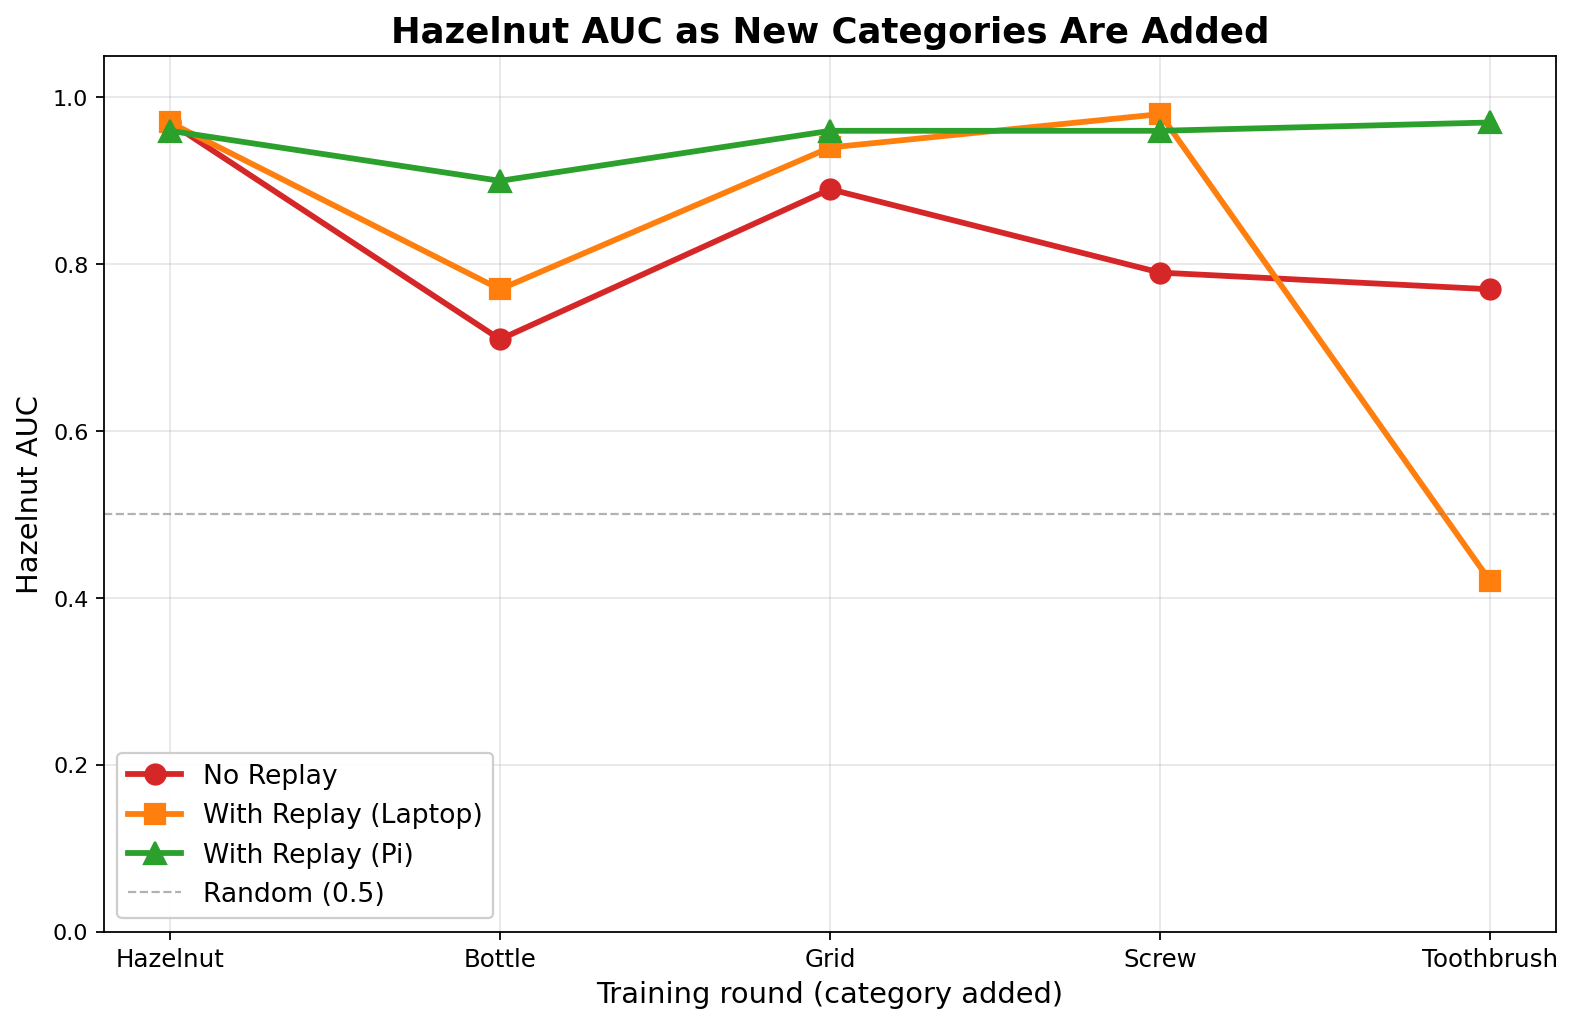
\includegraphics[width=0.7\textwidth]{auc_hazelnut_focus.png}
\caption{Hazelnut AUC across training rounds, comparing no-replay vs.
with-replay (laptop) vs. Raspberry Pi. Replay preserves the old category while
the no-replay baseline drifts.}
\label{fig:hazelnut}
\end{figure}

\subsection{Experiment 2: Feasibility and Timing on Raspberry Pi 5}
% Repeat the motif. The question: can the full train+infer pipeline run on the Pi,
% and what is the time cost vs. the laptop?
% TODO: present timing numbers (training sec, testing sec) and the Pi AUC table/plot.

\subsection{Findings and Discussion}
% Insights. Do the results support the hypothesis? Be honest about mixed/negative
% results - the template explicitly asks for this.
% TODO: e.g., replay clearly helps stability on some categories (Hazelnut, Screw)
% but the lambda / step-budget trade-off starves new categories in others; the Pi
% runs the same pipeline at higher wall-clock cost.

% ============================================================
% \section*{Acknowledgments}
% (Optional for project writeups - safe to leave commented out.)

% ============================================================
\begin{thebibliography}{9}

\bibitem{pellegrini2020latent}
L.~Pellegrini, G.~Graffieti, V.~Lomonaco, and D.~Maltoni,
``Latent Replay for Real-Time Continual Learning,''
\textit{IEEE/RSJ International Conference on Intelligent Robots and Systems (IROS)}, 2020.

\bibitem{bergmann2019mvtec}
P.~Bergmann, M.~Fauser, D.~Sattlegger, and C.~Steger,
``MVTec AD --- A Comprehensive Real-World Dataset for Unsupervised Anomaly Detection,''
\textit{IEEE/CVF Conference on Computer Vision and Pattern Recognition (CVPR)}, 2019.

% TODO: add more references as needed.
\end{thebibliography}

\end{document}
